\chapter{Electronic Spectroscopy and Photophysics}\label{ch:b3:electronic-spectroscopy}

Under the ultraviolet lamp of a dark bar, a glass of tonic water glows a
pale, ghostly blue. The quinine it contains absorbs ultraviolet light, which
the eye cannot see, and gives part of it back a few nanoseconds later as
visible blue light. Absorption, a short life in an excited state, emission at
a longer wavelength, the energy that does not come back as light: the fate of
an excited molecule is a competition between processes with rate constants,
and its spectrum is shaped by the vibrations of the molecule and by the
symmetry rules of \cref{ch:b3:group-theory-applied}. This chapter studies
electronic transitions and what happens after them, the subject called
photophysics; \cref{ch:b3:photochemistry} adds the cases in which the excited
molecule reacts.

\begin{recall}
The Year 1 volume measured absorbance with the Beer--Lambert law, $A =
\varepsilon\ell c$, defined the molar absorption coefficient, chromophores and
conjugated systems, and related colour to the absorption maximum. The Year 2
volume named the frontier orbitals HOMO and LUMO. \Cref{ch:b3:many-electron-atoms}
defined singlet and \omterm{def:b3:many-electron-atoms:singlet-triplet}{triplet states}; \cref{ch:b3:group-theory-applied} the
vanishing-integral theorem; \cref{ch:b3:rovibrational-spectroscopy} the
vibrational levels of a bond.
\end{recall}

\begin{omfigure}
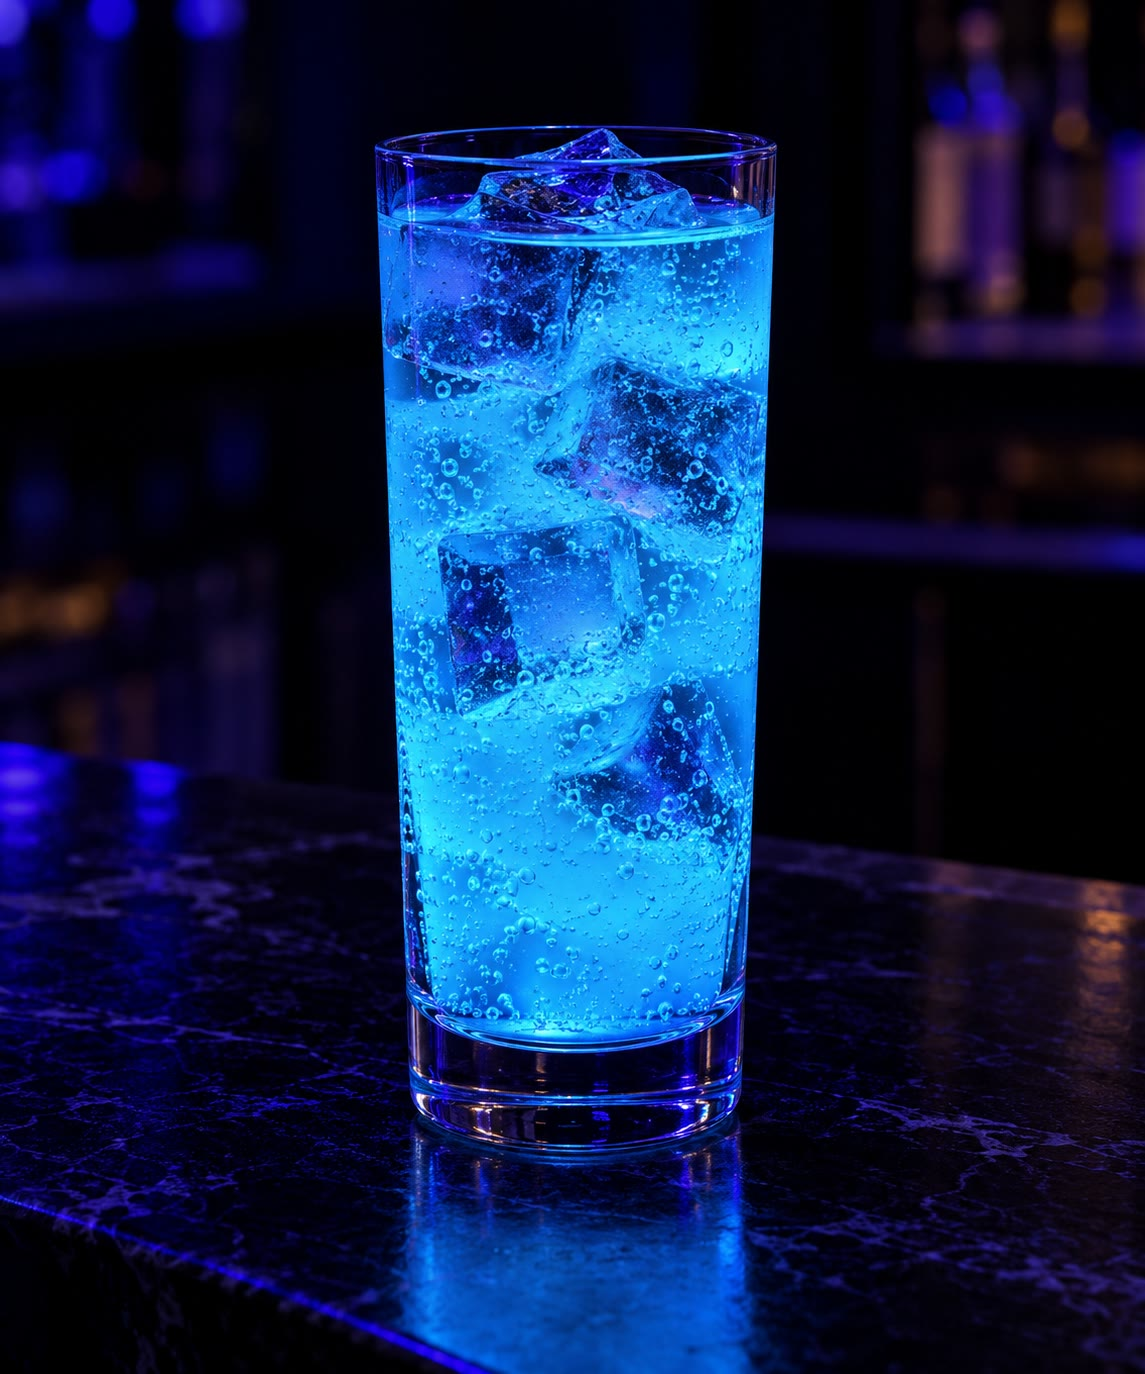
\includegraphics[height=4.6cm]{images/book4/ai/b3-07-tonic.jpg}\hspace{1em}%
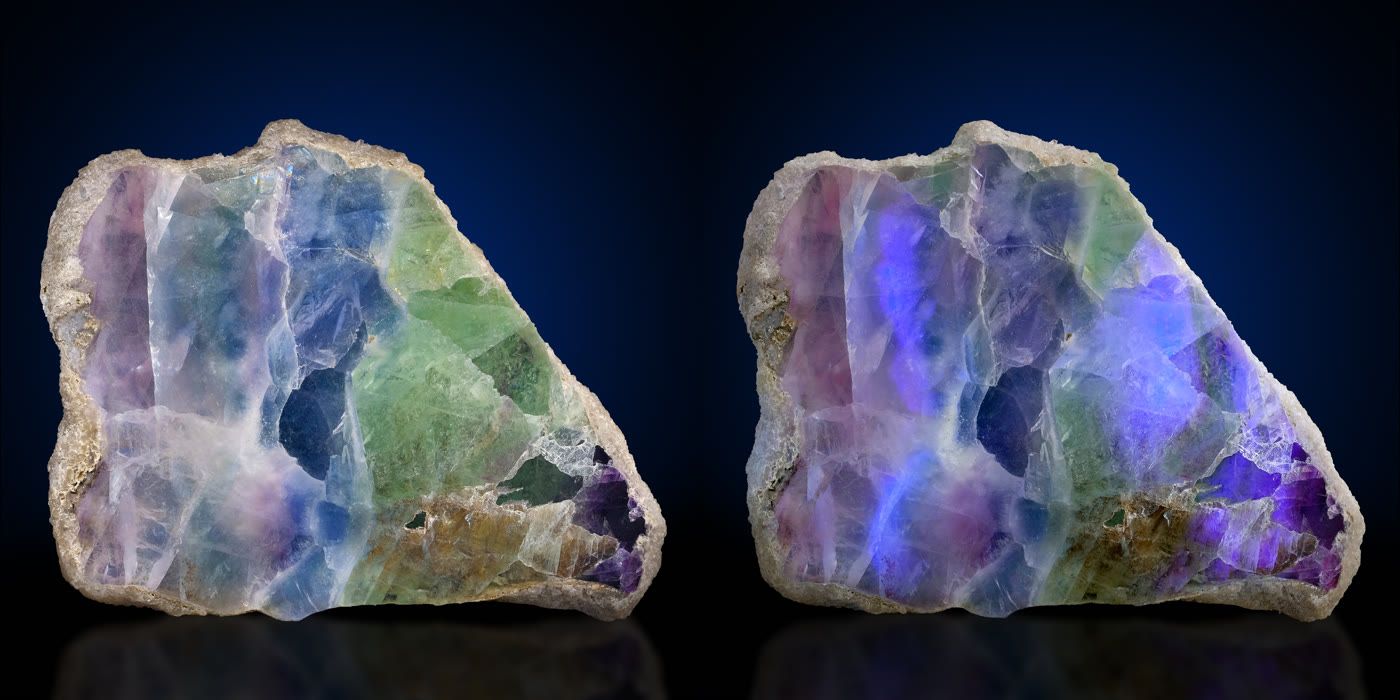
\includegraphics[height=4.6cm]{images/book4/fluorite-uv.jpg}

{\small Left: tonic water glowing blue under an ultraviolet lamp. Right:
fluorite in daylight and fluorescing under ultraviolet light; the mineral
gave \omterm{def:b3:electronic-spectroscopy:luminescence}{fluorescence} its name. Photograph Masha Milshina, CC BY 4.0.}
\end{omfigure}

\section{Electronic transitions and their selection rules}

\begin{definition}[Transition dipole moment, oscillator strength]\label{def:b3:electronic-spectroscopy:transition-dipole}
The \emph{transition dipole moment}\index{transition dipole moment} between
states $\Psi_i$ and $\Psi_f$ is $\boldsymbol\mu_{fi} = \langle\Psi_f|\hat{\boldsymbol\mu}|\Psi_i
\rangle$, with $\hat{\boldsymbol\mu} = -e\sum_k\mathbf r_k$ (plus the nuclear
charges, which cancel between orthogonal states). The \emph{oscillator
strength}\index{oscillator strength} $f$ is the dimensionless measure of the
intensity of a band, about 1 for the strongest transitions.
\end{definition}

\begin{proposition}[Intensity and oscillator strength]\label{prop:b3:electronic-spectroscopy:intensity}
The integrated absorption of a band is proportional to $|\boldsymbol\mu_{fi}|^2$,
and in practice
\[
f \approx 4.32\times10^{-9}\int\varepsilon(\tilde\nu)\,\dd\tilde\nu,
\]
with $\varepsilon$ in \unit{L.mol^{-1}.cm^{-1}} and $\tilde\nu$ in \unit{cm^{-1}}.
\end{proposition}
\admitted

The proportionality comes from time-dependent perturbation theory and the
numerical factor from the classical oscillator; both are treated in more
advanced courses. What matters here is that $f$ is large only when
$\boldsymbol\mu_{fi}$ is, and that symmetry can force it to zero.

\begin{theorem}[The spin selection rule]\label{thm:b3:electronic-spectroscopy:spin-rule}
An electric-dipole transition between states of different total spin is
forbidden: $\Delta S = 0$.
\end{theorem}

\begin{proof}
Each state is a product of a spatial and a spin function, $\Psi = \phi\,\chi$.
The dipole \omterm{def:b3:quantum-model-systems:operator}{operator} acts on positions only, so $\langle\phi_f\chi_f|\hat{\boldsymbol\mu}|
\phi_i\chi_i\rangle = \langle\phi_f|\hat{\boldsymbol\mu}|\phi_i\rangle\langle\chi_f|\chi_i\rangle$.
Spin functions of different $S$ are \omterm{def:b3:quantum-model-systems:operator}{eigenfunctions} of $\hat S^2$ with different
\omterm{def:b3:quantum-model-systems:operator}{eigenvalues}, hence orthogonal (\cref{thm:b3:quantum-model-systems:hermitian-real}):
the second factor vanishes.
\end{proof}

\begin{theorem}[The Laporte rule]\label{thm:b3:electronic-spectroscopy:laporte}
In a molecule with a \omterm{def:b3:point-groups:inversion}{centre of inversion}, an electric-dipole transition must
change parity: $g \leftrightarrow u$ is allowed, $g \leftrightarrow g$ and $u
\leftrightarrow u$ are forbidden. This is the \emph{Laporte rule}\index{Laporte
rule}.
\end{theorem}

\begin{proof}
The components of $\hat{\boldsymbol\mu}$ change sign under inversion: they are $u$.
The product $\Gamma_f\otimes\Gamma_\mu\otimes\Gamma_i$ is $g$ only if $\Gamma_f$ and $\Gamma_i$
have opposite parities; otherwise it is $u$ and cannot contain the \omterm{def:b3:group-theory-applied:reducible}{totally
symmetric representation} (\cref{thm:b3:group-theory-applied:vanishing-integral}).
\end{proof}

The two rules are strict for the idealised states; real molecules relax them
--- \omterm{def:b3:many-electron-atoms:spin-orbit}{spin--orbit coupling} mixes singlet and triplet character, vibrations
remove the centre of symmetry for an instant --- and the ``forbidden''
transitions appear, weakly. The $d$--$d$ bands of octahedral complexes, Laporte
forbidden and weak, owe their colour to this relaxation
(\cref{ch:b3:complex-spectra-magnetism}).

\begin{definition}[Charge-transfer transition]\label{def:b3:electronic-spectroscopy:charge-transfer}
A \emph{charge-transfer transition}\index{charge-transfer transition} moves an
electron from an orbital located mainly on one part of a system (a donor) to
an orbital located mainly on another (an acceptor); its transition dipole is
large, its band intense and broad, and its energy sensitive to the polarity of
the solvent.
\end{definition}

\begin{method}[Assigning an absorption band]\label{met:b3:electronic-spectroscopy:assign-band}
\begin{enumerate}
  \item $\varepsilon_{\max}$ above about \qty{e4}{L.mol^{-1}.cm^{-1}}: an allowed
        transition ($\pi\to\pi^*$ of a conjugated system, or charge transfer).
  \item $\varepsilon_{\max}$ of 10 to a few hundred: a forbidden one ($n\to\pi^*$,
        symmetry-forbidden; $d$--$d$, Laporte-forbidden).
  \item $\varepsilon_{\max}$ below 1: spin-forbidden.
  \item An $n\to\pi^*$ band moves to shorter wavelengths in protic solvents
        (the lone pair is stabilised by hydrogen bonds), a $\pi\to\pi^*$ band
        usually to longer ones.
\end{enumerate}
\end{method}

\section{The Franck--Condon principle}

\begin{theorem}[Franck--Condon principle]\label{thm:b3:electronic-spectroscopy:franck-condon}
Within the \omterm{def:b3:computational-chemistry:born-oppenheimer}{Born--Oppenheimer approximation}, and if the transition dipole
depends little on the nuclear positions, the intensity of the \omterm{def:b3:electronic-spectroscopy:vibronic}{vibronic
transition} from vibrational level $v''$ of the lower electronic state to level
$v'$ of the upper one is proportional to $|\langle\chi_{v'}|\chi_{v''}\rangle|^2$, the
square of the overlap of the two vibrational wavefunctions: this is the
\emph{Franck--Condon principle}\index{Franck--Condon principle}. Electronic
transitions are vertical: the nuclei do not move while the electrons jump.
\end{theorem}

\begin{proof}
With $\Psi = \psi_{\mathrm{el}}(\mathbf r;R)\chi_v(R)$, the transition moment is
$\int\chi_{v'}^*\big[\int\psi'^*_{\mathrm{el}}\hat\mu\psi''_{\mathrm{el}}\dd\mathbf r\big]
\chi_{v''}\,\dd R$. The bracket is the electronic transition moment
$\mu_{\mathrm{el}}(R)$; taken as constant (the Condon approximation), it comes out of
the integral, leaving $\mu_{\mathrm{el}}\langle\chi_{v'}|\chi_{v''}\rangle$.
\end{proof}

\begin{definition}[Vibronic transition, progression, Franck--Condon factor]\label{def:b3:electronic-spectroscopy:vibronic}
A \emph{vibronic transition}\index{vibronic transition} changes the electronic
and vibrational states together; the lines $v' \leftarrow 0$ for $v' = 0, 1, 2,
\dots$ form a \emph{vibronic progression}\index{vibronic progression}; the
\emph{Franck--Condon factor}\index{Franck--Condon factor} of a vibronic line is
$|\langle\chi_{v'}|\chi_{v''}\rangle|^2$.
\end{definition}

\begin{proposition}[Displaced oscillators]\label{prop:b3:electronic-spectroscopy:displaced}
If both states are harmonic with the same frequency and the upper minimum is
displaced by $\Delta$ (in units of $\sqrt{\hbar/m\omega}$), the \omterm{def:b3:electronic-spectroscopy:vibronic}{Franck--Condon
factors} from $v'' = 0$ form a Poisson distribution,
$|\langle v'|0\rangle|^2 = \eu^{-S}S^{v'}/v'!$, with $S = \Delta^2/2$; the strongest line
is near $v' = S$.
\end{proposition}
\admitted

The general proof uses the \omterm{def:b3:quantum-model-systems:ladder}{ladder operators} of
\cref{ch:b3:quantum-model-systems}; this chapter's figure data checks the
formula against direct integration. A small displacement gives one strong
0--0 line; a large one a long progression whose strongest member is far from
the 0--0 line.

\begin{omfigure}
\begin{tikzpicture}
\begin{axis}[name=pc, width=0.46\linewidth, height=6cm, xmin=-4, xmax=5, ymin=0,
  ymax=14, axis lines=left, xtick=\empty, ytick=\empty, xlabel={nuclear coordinate},
  ylabel={energy}, label style={font=\small}]
\addplot[black, thick] table[x=y, y=ground] {figdata/out/bachelor-3-franck-condon-curves.dat};
\addplot[omDef, thick] table[x=y, y=excited] {figdata/out/bachelor-3-franck-condon-curves.dat};
\draw[omabs] (axis cs:0,0.5) -- (axis cs:0,10.6);
\draw[omvib] (axis cs:-1,0.5) -- (axis cs:1,0.5);
\draw[omvib] (axis cs:0.732,9.5) -- (axis cs:2.732,9.5);
\draw[omvib] (axis cs:-0.000,10.5) -- (axis cs:3.464,10.5);
\draw[omvib] (axis cs:-0.504,11.5) -- (axis cs:3.968,11.5);
\draw[omvib] (axis cs:-0.914,12.5) -- (axis cs:4.378,12.5);
\node[font=\small, anchor=west] at (axis cs:-3.9,13.0) {excited};
\node[font=\small, anchor=west] at (axis cs:3.0,1.5) {ground};
\node[font=\scriptsize, anchor=east] at (axis cs:-0.05,5.5) {vertical};
\end{axis}
\begin{axis}[at={(pc.east)}, anchor=west, xshift=1.3cm, width=0.46\linewidth,
  height=6cm, xmin=-0.5, xmax=12.5, ymin=0, ymax=0.8, axis lines=left, ycomb,
  xlabel={$v'$}, ylabel={Franck--Condon factor}, label style={font=\small},
  tick label style={font=\small}]
\addplot[black, very thick] table[x=v, y=s03] {figdata/out/bachelor-3-franck-condon-sticks.dat};
\addplot[omDef, very thick, xshift=2pt] table[x=v, y=s15] {figdata/out/bachelor-3-franck-condon-sticks.dat};
\addplot[omThm, very thick, xshift=4pt] table[x=v, y=s5] {figdata/out/bachelor-3-franck-condon-sticks.dat};
\end{axis}
\end{tikzpicture}

{\small Left: a vertical transition from the lowest level of the ground state
lands where the excited curve, displaced to longer bond length, is high above
its minimum (drawn for $S = 1.5$). Right: \omterm{def:b3:electronic-spectroscopy:vibronic}{Franck--Condon factors} of the
progression for $S = 0.3$ (black), 1.5 (blue) and 5 (red); each set adds up
to 1.}
\end{omfigure}

\begin{example}[Iodine]\label{ex:b3:electronic-spectroscopy:iodine}
% ledger: diat:I2.re, diat:I2B.re, diat:I2B.we, imass:I127
Iodine vapour is violet because its B$\leftarrow$X band absorbs yellow-green light.
The bond lengthens from \qty{266.6}{pm} in the ground state to \qty{302.5}{pm} in
the B state. In the displaced-oscillator model with the B-state frequency
(\qty{125.7}{cm^{-1}}), $\Delta R = \qty{35.8}{pm}$ gives $S \approx 15$: the absorption is a
long progression whose strongest lines end on high vibrational levels of the
B state, and whose continuation runs into the dissociation continuum.
\end{example}

\section{The fates of an excited state: the Jablonski diagram}

\begin{definition}[Jablonski diagram]\label{def:b3:electronic-spectroscopy:jablonski}
A \emph{Jablonski diagram}\index{Jablonski diagram} shows the electronic states
of a molecule (singlets $S_0, S_1, S_2, \dots$ in one column, triplets $T_1, T_2,
\dots$ in another), their vibrational levels, and the processes connecting them:
radiative ones as straight arrows, radiationless ones as wavy arrows.
\end{definition}

\begin{definition}[Radiationless processes]\label{def:b3:electronic-spectroscopy:radiationless}
\emph{Vibrational relaxation}\index{vibrational relaxation} brings an excited
molecule to the lowest vibrational level of its electronic state by
collisions, in picoseconds. \emph{Internal conversion}\index{internal
conversion} is a radiationless transition between states of the same
multiplicity ($S_2 \to S_1$, $S_1 \to S_0$); \emph{intersystem
crossing}\index{intersystem crossing} one between states of different
multiplicity ($S_1 \to T_1$, $T_1 \to S_0$).
\end{definition}

\begin{definition}[Luminescence, fluorescence, phosphorescence, Stokes shift]\label{def:b3:electronic-spectroscopy:luminescence}
\emph{Luminescence}\index{luminescence} is emission of light by an excited
molecule. \emph{Fluorescence}\index{fluorescence} is spin-allowed emission,
usually $S_1 \to S_0$, fast (nanoseconds); \emph{phosphorescence}\index{phosphorescence}
is spin-forbidden emission, usually $T_1 \to S_0$, slow (milliseconds to
seconds). The \emph{Stokes shift}\index{Stokes shift} is the difference between
the absorption and emission maxima, in energy.
\end{definition}

\begin{omfigure}
\begin{tikzpicture}[font=\small, >=Stealth]
  \foreach \y/\l in {0/{$S_0$}, 3.4/{$S_1$}, 5.6/{$S_2$}}{
    \draw[omstate] (0,\y) -- (3.6,\y); \node[anchor=east] at (-0.1,\y) {\l};
    \foreach \d in {0.25,0.5,0.75}{\draw[omvib] (0,\y+\d) -- (3.6,\y+\d);}}
  \draw[omstate] (5.0,2.5) -- (7.6,2.5); \node[anchor=west] at (7.7,2.5) {$T_1$};
  \foreach \d in {0.25,0.5,0.75}{\draw[omvib] (5.0,2.5+\d) -- (7.6,2.5+\d);}
  \draw[omabs] (0.3,0) -- (0.3,4.15) node[pos=0.35, left, font=\scriptsize, align=right] {absorption};
  \draw[omabs] (0.7,0) -- (0.7,5.85);
  \draw[omnonrad] (1.05,5.85) -- (1.05,5.6);
  \draw[omnonrad] (1.05,5.6) -- (1.05,3.4) node[pos=0.5, right, font=\scriptsize] {IC};
  \draw[omnonrad] (0.45,4.15) -- (0.45,3.42);
  \draw[omfluo] (1.7,3.4) -- (1.7,0.5) node[pos=0.5, right, font=\scriptsize, align=left] {fluor-\\escence};
  \draw[omnonrad] (3.2,3.4) -- (3.2,0.02) node[pos=0.5, right, font=\scriptsize] {IC};
  \draw[omisc] (3.6,3.4) -- (5.0,3.1) node[pos=0.5, above, font=\scriptsize] {ISC};
  \draw[omnonrad] (5.3,3.1) -- (5.3,2.52);
  \draw[omphos] (6.0,2.5) -- (6.0,0.5) node[pos=0.5, right, font=\scriptsize, align=left] {phosphor-\\escence};
  \draw[omisc] (5.6,2.5) -- (3.7,0.02) node[pos=0.45, above left, font=\scriptsize, inner sep=1pt] {ISC};
  \draw[omvib, dashed] (3.6,0.5) -- (6.0,0.5);
  \draw[omvib, dashed] (3.6,0.0) -- (7.6,0.0);
\end{tikzpicture}

{\small A \omterm{def:b3:electronic-spectroscopy:jablonski}{Jablonski diagram}. Straight arrows: absorption (blue), \omterm{def:b3:electronic-spectroscopy:luminescence}{fluorescence}
(red), \omterm{def:b3:electronic-spectroscopy:luminescence}{phosphorescence} (orange); wavy arrows: \omterm{def:b3:electronic-spectroscopy:radiationless}{vibrational relaxation} and
\omterm{def:b3:electronic-spectroscopy:radiationless}{internal conversion} (IC); dashed wavy arrows: \omterm{def:b3:electronic-spectroscopy:radiationless}{intersystem crossing} (ISC).
Emission starts from the lowest vibrational level of $S_1$ or $T_1$ and may end
on any level of $S_0$.}
\end{omfigure}

\begin{proposition}[Kasha's rule]\label{prop:b3:electronic-spectroscopy:kasha}
\omterm{def:b3:electronic-spectroscopy:luminescence}{Luminescence} occurs, with very few exceptions, from the lowest excited state
of a given multiplicity ($S_1$ or $T_1$), whatever state was first excited:
\emph{Kasha's rule}\index{Kasha's rule}.
\end{proposition}
\begin{proof}[Status]
Established experimentally; the reason is that \omterm{def:b3:electronic-spectroscopy:radiationless}{internal conversion} between
upper excited states, which lie close together, is far faster than emission,
while the gap $S_1$--$S_0$ is large.
\end{proof}

\begin{proposition}[Mirror image]\label{prop:b3:electronic-spectroscopy:mirror}
If the excited and ground states have similar vibrational structure, the
\omterm{def:b3:electronic-spectroscopy:luminescence}{fluorescence} band is the mirror image of the first absorption band about their
common 0--0 line; the emission lies at longer wavelengths (\omterm{def:b3:electronic-spectroscopy:luminescence}{Stokes shift}).
\end{proposition}

\begin{proof}
Absorption goes from $v'' = 0$ to the levels $v'$ of $S_1$, at $E_{00} + v'h\nu'$; emission
from $v' = 0$ to the levels $v''$ of $S_0$, at $E_{00} - v''h\nu''$. With equal
frequencies and the same \omterm{def:b3:electronic-spectroscopy:vibronic}{Franck--Condon factors} (equal displacement), the two
progressions are symmetric about $E_{00}$.
\end{proof}

\begin{omfigure}
\begin{tikzpicture}
\begin{axis}[width=0.75\linewidth, height=5cm, xmin=17, xmax=33, ymin=0,
  ymax=1.15, axis x line=bottom, axis y line=left, ytick=\empty,
  xlabel={wavenumber / $10^3$ cm$^{-1}$}, ylabel={intensity},
  legend cell align=left, legend style={font=\small, draw=none, at={(0.02,0.97)}, anchor=north west},
  tick label style={font=\small}, label style={font=\small}]
\addplot[omDef, thick] table[x=nu, y=abs] {figdata/out/bachelor-3-photophysics-bands.dat};
\addlegendentry{absorption}
\addplot[omThm, thick] table[x=nu, y=em] {figdata/out/bachelor-3-photophysics-bands.dat};
\addlegendentry{fluorescence}
\draw[gray, dashed] (axis cs:25,0) -- (axis cs:25,1.12);
\node[font=\scriptsize, gray, anchor=south west] at (axis cs:25,1.0) {0--0};
\end{axis}
\end{tikzpicture}

{\small Absorption and \omterm{def:b3:electronic-spectroscopy:luminescence}{fluorescence} of a model molecule ($S = 1$, vibrational
quantum \qty{1400}{cm^{-1}}): mirror images about the 0--0 line; the maxima are
separated by the \omterm{def:b3:electronic-spectroscopy:luminescence}{Stokes shift}.}
\end{omfigure}

\section{Kinetics of excited states}

After excitation, the population of $S_1$ decays by every process open to it,
each first order: radiative decay $k_r$, \omterm{def:b3:electronic-spectroscopy:radiationless}{internal conversion} $k_{\mathrm{IC}}$,
\omterm{def:b3:electronic-spectroscopy:radiationless}{intersystem crossing} $k_{\mathrm{ISC}}$.

\begin{definition}[Excited-state lifetime, radiative lifetime]\label{def:b3:electronic-spectroscopy:lifetime}
The \emph{excited-state lifetime}\index{excited-state lifetime} is $\tau =
1/\sum k$, the time constant of the exponential decay of the excited
population. The \emph{radiative lifetime}\index{radiative lifetime} $\tau_r =
1/k_r$ is the lifetime the state would have if emission were its only
fate.
\end{definition}

\begin{definition}[Quantum yield]\label{def:b3:electronic-spectroscopy:quantum-yield}
The \emph{quantum yield}\index{quantum yield} of a process that follows the
absorption of light is the number of events of that process divided by the
number of photons absorbed. The \emph{fluorescence quantum
yield}\index{fluorescence quantum yield} $\Phi_F$ is the number of photons
emitted as \omterm{def:b3:electronic-spectroscopy:luminescence}{fluorescence} per photon absorbed.
\end{definition}

\begin{proposition}[Quantum yield and lifetime]\label{prop:b3:electronic-spectroscopy:quantum-yield}
$\Phi_F = k_r/(k_r + k_{\mathrm{IC}} + k_{\mathrm{ISC}}) = k_r\tau = \tau/\tau_r$; likewise
$\Phi_{\mathrm{ISC}} = k_{\mathrm{ISC}}\tau$, and the yields of the competing processes add
up to 1.
\end{proposition}

\begin{proof}
$\dd[S_1]/\dd t = -(k_r + k_{\mathrm{IC}} + k_{\mathrm{ISC}})[S_1]$, so $[S_1] = [S_1]_0\eu^{-t/\tau}$.
The number of photons emitted is $\int_0^\infty k_r[S_1]\,\dd t = k_r\tau[S_1]_0$, out of
$[S_1]_0$ excited molecules. The same integral with each $k$ gives each yield,
and their sum is $\tau\sum k = 1$.
\end{proof}

\begin{definition}[Fluorescence quencher, dynamic and static quenching]\label{def:b3:electronic-spectroscopy:quencher}
A \emph{fluorescence quencher}\index{fluorescence quencher} is a species that
reduces \omterm{def:b3:electronic-spectroscopy:luminescence}{fluorescence}. In \emph{dynamic quenching}\index{dynamic quenching} it
deactivates the excited molecule on collision, adding a rate $k_q[Q]$ and
shortening the lifetime; in \emph{static quenching}\index{static quenching} it
forms a non-fluorescent complex with the ground-state molecule, reducing the
intensity without changing the lifetime of the molecules that still emit.
\end{definition}

\begin{theorem}[Stern--Volmer equation]\label{thm:b3:electronic-spectroscopy:stern-volmer}
For \omterm{def:b3:electronic-spectroscopy:quencher}{dynamic quenching},
\[
\frac{I_0}{I} = \frac{\tau_0}{\tau} = 1 + k_q\tau_0[Q] = 1 + K_{SV}[Q],
\]
the \emph{Stern--Volmer equation}\index{Stern--Volmer equation}, where $I_0$, $\tau_0$
are measured without quencher and $K_{SV} = k_q\tau_0$.
\end{theorem}

\begin{proof}
With quencher, $\tau = 1/(k_0 + k_q[Q])$ with $k_0 = 1/\tau_0$, so $\tau_0/\tau = 1 +
k_q\tau_0[Q]$. The intensity is proportional to $\Phi_F = k_r\tau$, so $I_0/I = \tau_0/\tau$.
\end{proof}

\begin{omfigure}
\begin{tikzpicture}
\begin{axis}[name=dec, width=0.5\linewidth, height=5cm, xmin=0, xmax=40, ymode=log,
  ymin=0.005, ymax=1.2, axis lines=left, xlabel={$t$ / ns}, ylabel={$I(t)/I(0)$},
  legend cell align=left, legend style={font=\scriptsize, draw=none, at={(0.98,0.98)}, anchor=north east},
  tick label style={font=\small}, label style={font=\small}]
\addplot[black, thick] table[x=t, y=q0] {figdata/out/bachelor-3-photophysics-decays.dat};
\addlegendentry{$[Q] = 0$}
\addplot[omDef, thick] table[x=t, y=q1] {figdata/out/bachelor-3-photophysics-decays.dat};
\addlegendentry{0.01 M}
\addplot[omProp, thick] table[x=t, y=q2] {figdata/out/bachelor-3-photophysics-decays.dat};
\addlegendentry{0.02 M}
\addplot[omThm, thick] table[x=t, y=q4] {figdata/out/bachelor-3-photophysics-decays.dat};
\addlegendentry{0.04 M}
\end{axis}
\begin{axis}[at={(dec.east)}, anchor=west, xshift=1.4cm, width=0.42\linewidth,
  height=5cm, xmin=0, xmax=0.045, ymin=0, ymax=3.3, axis lines=left,
  xlabel={$[Q]$ / mol L$^{-1}$}, ylabel={$I_0/I = \tau_0/\tau$},
  xticklabel style={/pgf/number format/fixed, /pgf/number format/precision=2},
  scaled x ticks=false, tick label style={font=\small}, label style={font=\small}]
\addplot[omThm, thick, mark=*] table[x=Q, y=I0I] {figdata/out/bachelor-3-photophysics-sv.dat};
\end{axis}
\end{tikzpicture}

{\small \omterm{def:b3:electronic-spectroscopy:quencher}{Dynamic quenching} of a model fluorophore ($\tau_0 = \qty{10}{ns}$, $k_q =
\qty{5e9}{L.mol^{-1}.s^{-1}}$). Left: \omterm{def:b3:electronic-spectroscopy:luminescence}{fluorescence} decays, straight lines on a log
scale, steeper with more quencher. Right: the Stern--Volmer line, of slope
$K_{SV} = k_q\tau_0 = \qty{50}{L/mol}$.}
\end{omfigure}

\begin{method}[Relative fluorescence quantum yield]\label{met:b3:electronic-spectroscopy:relative-yield}
\begin{enumerate}
  \item Choose a standard of known $\Phi_{\mathrm{std}}$ absorbing at the same
        excitation wavelength.
  \item Prepare dilute solutions ($A < 0.1$, to avoid re-absorption) and record
        their absorbances $A$ and integrated emission spectra $F$ under identical
        conditions.
  \item $\Phi = \Phi_{\mathrm{std}}\,\dfrac{F}{F_{\mathrm{std}}}\,\dfrac{A_{\mathrm{std}}}{A}\,
        \dfrac{n^2}{n_{\mathrm{std}}^2}$, the last factor correcting for the refractive
        indices of the solvents.
\end{enumerate}
\end{method}

\begin{method}[Analysing quenching data]\label{met:b3:electronic-spectroscopy:stern-volmer}
\begin{enumerate}
  \item Plot $I_0/I$ against $[Q]$; a straight line through 1 gives $K_{SV}$.
  \item Measure lifetimes too: if $\tau_0/\tau$ follows the same line, the quenching
        is dynamic, and $k_q = K_{SV}/\tau_0$; if $\tau$ does not change, it is static.
  \item Compare $k_q$ with the diffusion limit, about \qty{e10}{L.mol^{-1}.s^{-1}} in
        water (\cref{ch:b3:rate-theories}): a $k_q$ close to it means nearly every
        encounter quenches.
\end{enumerate}
\end{method}

\begin{example}[Quinine and anthracene]\label{ex:b3:electronic-spectroscopy:quinine}
% ledger: fl:quinine.labs, fl:quinine.eps, fl:quinine.phi, fl:anthracene.labs, fl:anthracene.phi
Quinine sulfate in \qty{0.5}{M} sulfuric acid absorbs at \qty{349}{nm} with $\varepsilon =
\qty{5700}{L.mol^{-1}.cm^{-1}}$ and fluoresces with $\Phi_F = 0.546$, which makes it the
classic standard for relative \omterm{def:b3:electronic-spectroscopy:quantum-yield}{quantum yields}. Anthracene in cyclohexane
absorbs at \qty{356}{nm} and has $\Phi_F = 0.36$; most of the rest of its excited
molecules cross to the triplet.
\end{example}

\section{Applications}

\omterm{def:b3:electronic-spectroscopy:luminescence}{Fluorescence} is detected against a dark background, which makes fluorimetry
a hundred to a thousand times more sensitive than absorption spectroscopy:
nanomolar concentrations of a fluorescent compound are measured routinely.
Fluorescent probes report on their surroundings through their wavelength,
yield or lifetime (polarity, pH, the binding of an ion); energy transfer
between two fluorophores, efficient only over a few nanometres, measures
distances in proteins. Phosphorescent complexes of heavy metals, in which
\omterm{def:b3:many-electron-atoms:spin-orbit}{spin--orbit coupling} makes \omterm{def:b3:electronic-spectroscopy:radiationless}{intersystem crossing} efficient, harvest triplets
in the light-emitting diodes of display screens.

\begin{inthelab}[Time-correlated single-photon counting]
To measure a nanosecond lifetime, the sample is excited by a pulsed laser
diode at a megahertz repetition rate, and for each pulse the delay of the
first \omterm{def:b3:electronic-spectroscopy:luminescence}{fluorescence} photon detected is recorded. After millions of pulses the
histogram of delays is the decay curve, from which $\tau$ is fitted, with the
instrument response measured on a scattering solution. The ultraviolet
source is enclosed; the operator works with goggles that block its
wavelength.
\end{inthelab}

\begin{history}[Stokes, 1852]
George Gabriel Stokes passed sunlight through a violet glass and a prism
into a solution of quinine, and saw blue light emerge from the region lit by
invisible ultraviolet rays: the emitted light always had a longer wavelength
than the light absorbed. He called the phenomenon \omterm{def:b3:electronic-spectroscopy:luminescence}{fluorescence}, after the
mineral fluorite, which glows the same way.
\end{history}

\section{Exercises}

\begin{exercise}[$\star$]\label{exo:b3:electronic-spectroscopy:1}
Allowed or forbidden, and by which rule: (a) $S_0 \to T_1$ in benzene; (b) a $d$--$d$
transition of an octahedral complex; (c) the $\pi\to\pi^*$ transition of ethene
($B_{1u} \leftarrow A_g$ in $D_{2h}$); (d) the $n\to\pi^*$ transition of methanal
($A_2$)?
\end{exercise}

\begin{exercise}[$\star$]\label{exo:b3:electronic-spectroscopy:2}
A compound absorbs at \qty{349}{nm} and fluoresces with a maximum at
\qty{450}{nm} (data of the exercise). Compute the \omterm{def:b3:electronic-spectroscopy:luminescence}{Stokes shift} in \unit{cm^{-1}} and in
eV.
\end{exercise}

\begin{exercise}[$\star$]\label{exo:b3:electronic-spectroscopy:3}
% ledger: fl:quinine.eps
Compute the absorbance at \qty{349}{nm} of a \qty{1.0e-5}{mol/L} quinine sulfate
solution in a \qty{1}{cm} cell, and the fraction of the light it absorbs.
\end{exercise}

\begin{exercise}[$\star$]\label{exo:b3:electronic-spectroscopy:4}
A fluorophore has $\Phi_F = 0.60$ and $\tau = \qty{4.0}{ns}$. Compute $k_r$, the
\omterm{def:b3:electronic-spectroscopy:lifetime}{radiative lifetime} and the sum of the non-radiative rate constants.
\end{exercise}

\begin{exercise}[$\star\star$]\label{exo:b3:electronic-spectroscopy:5}
A band is Gaussian with $\varepsilon_{\max} = \qty{5700}{L.mol^{-1}.cm^{-1}}$ and a full width at
half maximum of \qty{5000}{cm^{-1}}. Estimate its \omterm{def:b3:electronic-spectroscopy:transition-dipole}{oscillator strength} (the integral
of a Gaussian is $1.0645\,\varepsilon_{\max}\times$FWHM).
\end{exercise}

\begin{exercise}[$\star\star$]\label{exo:b3:electronic-spectroscopy:6}
For displaced oscillators, find the strongest line of the progression for
$S = 0.3$, 1.5 and 5, and the ratio of its factor to that of the 0--0 line.
\end{exercise}

\begin{exercise}[$\star\star$]\label{exo:b3:electronic-spectroscopy:7}
From $S_1$, $k_r = \qty{1.0e8}{s^{-1}}$, $k_{\mathrm{IC}} = \qty{2.0e7}{s^{-1}}$ and $k_{\mathrm{ISC}} =
\qty{3.0e8}{s^{-1}}$. Compute $\tau$, $\Phi_F$ and $\Phi_{\mathrm{ISC}}$.
\end{exercise}

\begin{exercise}[$\star\star$]\label{exo:b3:electronic-spectroscopy:8}
% ledger: fl:quinine.phi, nD:water, nD:cyclohexane
The \omterm{def:b3:electronic-spectroscopy:luminescence}{fluorescence} of anthracene in cyclohexane ($A = 0.040$) integrates to 0.46
times that of quinine sulfate in dilute sulfuric acid ($A = 0.050$, $\Phi =
0.546$). With refractive indices 1.4266 (cyclohexane) and 1.333 (water, for the
dilute acid), compute $\Phi_F$ of anthracene.
\end{exercise}

\begin{exercise}[$\star\star$]\label{exo:b3:electronic-spectroscopy:9}
The lifetime of a fluorophore is 8.0, 5.6 and \qty{4.3}{ns} at quencher
concentrations 0, 0.010 and \qty{0.020}{mol/L}. Is the quenching dynamic? Find
$K_{SV}$ and $k_q$.
\end{exercise}

\begin{exercise}[$\star\star\star$]\label{exo:b3:electronic-spectroscopy:10}
Adding a quencher halves the \omterm{def:b3:electronic-spectroscopy:luminescence}{fluorescence} intensity while the measured
lifetime stays at \qty{6.0}{ns}. What kind of quenching is it, and what does it
imply about the ground state? Write the corresponding relation between $I_0/I$
and the association constant of the complex.
\end{exercise}

\begin{exercise}[$\star\star\star$]\label{exo:b3:electronic-spectroscopy:11}
% ledger: fl:anthracene.phi
Anthracene in cyclohexane has $\Phi_F = 0.36$ and, in the conditions of a
measurement, $\tau = \qty{5.0}{ns}$ (data of the exercise). Compute $\tau_r$, and the
yield of the triplet if \omterm{def:b3:electronic-spectroscopy:radiationless}{internal conversion} is negligible. Why is the
\omterm{def:b3:electronic-spectroscopy:lifetime}{radiative lifetime} longer than the measured one?
\end{exercise}

\begin{exercise}[$\star\star\star$]\label{exo:b3:electronic-spectroscopy:12}
For two electrons, the singlet spin function is $\frac{1}{\sqrt2}[\alpha\beta - \beta\alpha]$
and the $M_S = 0$ triplet function $\frac{1}{\sqrt2}[\alpha\beta + \beta\alpha]$. Show that
they are orthogonal, and conclude on the intensity of $T_1 \leftarrow S_0$ in the
absence of \omterm{def:b3:many-electron-atoms:spin-orbit}{spin--orbit coupling}.
\end{exercise}

\section{Problem: Why Tonic Water Glows}

\begin{problem}[{Weekend problem --- absorption by quinine, the fate of its
excited state, quenching by chloride ions, and whether every encounter
quenches}]
\label{pb:b3:electronic-spectroscopy:1}
% ledger: fl:quinine.labs, fl:quinine.eps, fl:quinine.phi, visc:H2O.25C
Quinine sulfate in \qty{0.5}{M} sulfuric acid: absorption maximum \qty{349}{nm},
$\varepsilon = \qty{5700}{L.mol^{-1}.cm^{-1}}$, $\Phi_F = 0.546$. Data of the problem: the
\omterm{def:b3:electronic-spectroscopy:luminescence}{fluorescence} lifetime without quencher is $\tau_0 = \qty{19}{ns}$; the emission
maximum is near \qty{450}{nm}; adding sodium chloride gives the intensity ratios
\begin{center}\small
\begin{tabular}{lccccc}
\hline
$[\ce{Cl-}]$ / mol L$^{-1}$ & 0 & 0.010 & 0.020 & 0.040 & 0.080 \\
$I_0/I$ & 1.000 & 1.594 & 2.188 & 3.376 & 5.752 \\ \hline
\end{tabular}
\end{center}
Water at \qty{25}{\celsius} has viscosity \qty{0.890}{mPa.s}; $R =
\qty{8.314}{J.K^{-1}.mol^{-1}}$.

\medskip\noindent\textbf{Part I --- Absorption.}
\begin{enumerate}
  \item Compute the absorbance at \qty{349}{nm} of a \qty{1.0e-4}{mol/L} solution in a
        \qty{1}{cm} cell.
  \item What fraction of the incident light is absorbed?
  \item Is the transition allowed? Use $\varepsilon$.
  \item Give the energy of the absorbed photon in eV.
  \item Why does the eye see no absorption colour in tonic water?
  \item Why is a solution for \omterm{def:b3:electronic-spectroscopy:luminescence}{fluorescence} work kept below $A = 0.1$?
\end{enumerate}

\medskip\noindent\textbf{Part II --- The excited state.}
\begin{enumerate}[resume]
  \item Draw the \omterm{def:b3:electronic-spectroscopy:jablonski}{Jablonski diagram} of the processes from $S_1$.
  \item Compute the radiative rate constant $k_r$ and the \omterm{def:b3:electronic-spectroscopy:lifetime}{radiative lifetime}.
  \item Compute the total non-radiative rate constant.
  \item Compute the \omterm{def:b3:electronic-spectroscopy:luminescence}{Stokes shift} in \unit{cm^{-1}}.
  \item Why is the emission blue although the absorption is in the ultraviolet?
  \item What fraction of the absorbed energy leaves as \omterm{def:b3:electronic-spectroscopy:luminescence}{fluorescence}, counting
        the energy of each photon?
\end{enumerate}

\medskip\noindent\textbf{Part III --- Quenching by chloride.}
\begin{enumerate}[resume]
  \item Plot $I_0/I$ against $[\ce{Cl-}]$ and check that it is linear.
  \item Determine $K_{SV}$ by least squares through the five points.
  \item Assuming \omterm{def:b3:electronic-spectroscopy:quencher}{dynamic quenching}, compute $k_q$.
  \item What lifetime would you measure at \qty{0.040}{mol/L}?
  \item How would you prove experimentally that the quenching is dynamic?
  \item Why is tonic water, which contains no chloride, a good place for
        quinine to glow?
\end{enumerate}

\medskip\noindent\textbf{Part IV --- Every encounter?}
\begin{enumerate}[resume]
  \item The rate constant of encounters controlled by diffusion in a solvent of
        viscosity $\eta$ is $k_d \approx 8RT/3\eta$. Compute it in \unit{L.mol^{-1}.s^{-1}}.
  \item Compare $k_q$ and $k_d$.
  \item What fraction of the encounters lead to quenching?
  \item Would the quenching be faster or slower in a more viscous solvent?
  \item State the result: the ratio $k_q/k_d$ for the quenching of quinine by
        chloride.
\end{enumerate}
\end{problem}
